% TEMPLATE FROM:
% NAME:		swift_scijust_template.tex
% Modified on 2/17/16 by Corey Mutnik

\documentclass[letterpaper,11pt]{article}
%\documentclass[letterpaper,11pt,twocolumn]{article

\usepackage{graphics,graphicx}
%\usepackage{psfig}
\usepackage{times}
\usepackage{float}		% allows use of 'H' command
%\usepackage[demo]{graphicx}
%\usepackage{caption}
\usepackage{subcaption}


\usepackage{hyperref}	% needed to add hyperlinks
\usepackage{url}		% for tilda symbol
\hypersetup{
  colorlinks=true,
  linkcolor=blue,
  filecolor=magenta,
  urlcolor=cyan,
  %pdfnewwindow=true,
}



%%%%%%%%%%%%%%%%%%%%%%%%%%%%%%%%%%%%%%%%%%%%%%%%%
%%%%% Page dimensions                       %%%%%
%%%%% DO NOT CHANGE THE FOLLOWING 9 LINES!  %%%%%
%%%%%%%%%%%%%%%%%%%%%%%%%%%%%%%%%%%%%%%%%%%%%%%%%

\setlength{\textwidth}{7in} 
\setlength{\textheight}{9.5in}
\setlength{\topmargin}{-0.2in} 
\setlength{\oddsidemargin}{-0.2in}
\setlength{\evensidemargin}{-0.2in} 
\setlength{\headheight}{0in}
\setlength{\headsep}{0in} 
\setlength{\hoffset}{0in}
\setlength{\voffset}{0in}


%%%%%%%%%%%%%%%%%%%%%%%%%%%%%%%%%%
%%%%% Section heading format %%%%%
%%%%%%%%%%%%%%%%%%%%%%%%%%%%%%%%%%

\makeatletter
\renewcommand{\section}{\@startsection%
{section}{1}{0mm}{-\baselineskip}%
{0.5\baselineskip}{\normalfont\Large\bfseries}}%
\makeatother



% DEFINE BOX ENVIRONMENT %%%%%%%%%%%%%%%%%%%%%%%%%%%%%%%%%%%%%%%%%%%%%%%%%%%%%%%%%%%%%%%%%%%%%%%%%%%%%%
%%%%%%%%%%%%%%%%%%%%%%%%%%%%%%%%%%%%%%%%%%%%%%%%%%%%%%%%%%%%%%%%%%%%%%%%%%%%%%%%%%%%%%%%%%%%%%%%%%%%%%%
\newsavebox\FrameBox
\newenvironment{Frame}{%
  \noindent\setbox\FrameBox\hbox\bgroup\minipage{1.01\textwidth}\parskip\baselineskip\ignorespaces
}{%
  \endminipage\egroup\fbox{\box\FrameBox}\par
}
%%%%%%%%%%%%%%%%%%%%%%%%%%%%%%%%%%%%%%%%%%%%%%%%%%%%%%%%%%%%%%%%%%%%%%%%%%%%%%%%%%%%%%%%%%%%%%%%%%%%%%%
%%%%%%%%%%%%%%%%%%%%%%%%%%%%%%%%%%%%%%%%%%%%%%%%%%%%%%%%%%%%%%%%%%%%%%%%%%%%%%%%%%%%%%%%%%%%%%%%%%%%%%%



\begin{document}
\pagestyle{plain}
\pagenumbering{arabic}

\begin{center} 
\bfseries\uppercase{\Large{University of Hawaii $\bullet$ Institute for Astronomy} \\ 
\large{Research Proposal -- Observing Time Request}}
\end{center}
\vspace{-0.3cm}


\iffalse
	% box around names, emails, and institution
	\noindent\fbox{\linespread{1.5}
		\parbox{\textwidth}{\bf{
				Names: {Daichi Hiramatsu} \& {Corey Mutnik} \\
				E-mails: dhiramat@hawaii.edu \& cmutnik@hawaii.edu\\
				Institution/Dept: UH
			}
		}
	} 
	~\\ %this is here to make gap between boxes
	% box around program titles
	\noindent\fbox{\linespread{1.5}
		\parbox{\textwidth}{\bf{
				Program Title\\
				A. Measuring the Milky Way\\
				B.\\
				C.
			}
		}
	} 
\fi


\noindent\fbox{\linespread{2}
  \parbox{\textwidth}{\bf{
	\begin{minipage}{0.5\textwidth}
		\begin{flushleft}
	    	\subsection*{Author$^{*}$~:~Daichi~Hiramatsu}
	    	%\subsection*{Author$_{1}$~:~Daichi~Hiramatsu\\E-mail$_{1}$~:~dhiramat@hawaii.edu}
		\end{flushleft}
	\end{minipage}
  \hfill
	\begin{minipage}{0.5\textwidth}
		\begin{flushright}
	    	\textbf{\large Author$^{\dagger}$~:~Corey Mutnik~~}\\[1.5cm]
		\end{flushright}
	\end{minipage}
	\begin{minipage}{0.5\textwidth}
		\begin{flushleft}
			\subsection*{E-mail$^{*}$~:~dhiramat@hawaii.edu}
		\end{flushleft}
	\end{minipage}
  \hfill
	\begin{minipage}{0.5\textwidth}
		\begin{flushright}
	    	\textbf{\large E-mail$^{\dagger}$~:~cmutnik@hawaii.edu~~}\\[1.5cm]
		\end{flushright}
	\end{minipage}

	\subsection*{Institution/Dept$^{*,\dagger}$~:~UH}
  }
 }
}

~\\~\\ % for gap between frames

\noindent\fbox{\linespread{1.5}
	\parbox{\textwidth}{\bf{
			Program Title\\
			A. Measuring the structure of the Milky Way spiral arms and testing a new method of distance measurement using ISM\\
			B.\\
			C.
		}
	}
} 

~\\~\\ % for gap between frames

\begin{Frame}
\noindent {\bf \\Abstract:}
Using various data reduction techniques, we will measure the structure and age of the Milky Way galaxy's spiral arms and test a new method of distance measurement using ISM. We request $90$~hours using Pathfinder to obtain g, r, and i imaging for variable stars in the galactic plane. From the spatial distribution of variable stars, we will determine the structure and age of spiral arms. From estimating amount of ISM near variable stars, we will test a distance measurement method to stars near variable stars.
% can report variable stars to AAVSO:
% \url{https://www.aavso.org/how-report-new-variable-star-discoveries}

\end{Frame}
~\\


\section*{TELESCOPE TIME REQUESTED}

\begin{table}[H]\label{tab:request-telescope-time}
	\begin{center}
		%\caption{\it \small{[title]}}
		\resizebox{\columnwidth}{!}{%
	\begin{tabular}{ | c | c | c | c | c | c | } \hline
		Run & Program & Telescope & Instrument & Nights (n) or hours (h) & Observers' initials \\ \hline
		1 & A & Pathfinder & & 15~n & DH \& CM \\ \hline
		%2 & ~ & ~ & ~ & ~ \\ \hline
		%3 & ~ & ~ & ~ & ~ \\ \hline
		%4 & ~ & ~ & ~ & ~ \\ \hline
		%5 & ~ & ~ & ~ & ~ \\ \hline
		%6 & ~ & ~ & ~ & ~ \\ \hline
		%7 & ~ & ~ & ~ & ~ \\ \hline
		%8 & ~ & ~ & ~ & ~ \\ \hline
		%9 & ~ & ~ & ~ & ~ \\ \hline
	\end{tabular}
	}
	\end{center}
\end{table}


\section*{COLLABORATORS}
\begin{table}[H]\label{tab:collabs}
	\begin{center}
		%\caption{\it \small{[title]}}
		\resizebox{\columnwidth}{!}{%
	\begin{tabular}{ | c | c | c | c | } \hline
		Name & Institution & E-mail & Program(s) \\ \hline
		 John L. Tonry & IfA & jt@ifa.hawaii.edu & A \\ \hline
		 Conor McPartland & IfA & conormcp@ifa.hawaii.edu & A \\ \hline
		 Marielle Dela Cruz & UH & msdelacr@hawaii.edu & A \\ \hline
		 Jeff Kleyner & UH & jeff2012@hawaii.edu & A \\ \hline
		 & & & \\ \hline
		 & & & \\ \hline
		 & & & \\ \hline
		 & & & \\ \hline
	\end{tabular}
	}
	\end{center}
\end{table}

\clearpage

\section{SCIENTIFIC JUSTIFICATION}

\subsection{Immediate Objective}
%located on the Milky Way galaxy. 
To determine the size and shape of particular spiral arms, variable star distributions must be spatially mapped.  
%Distributions of variable stars allows for the determination of both size and shape of 
In observed regions, the density of variable stars will give insight into the age (\textit{and star formation epoch?}) of our galaxy.  The distance to each star will be calculated using the distance modulus,
\begin{center}
$d = 10^{(m - M + 5)/5},$
\end{center}
where d is the distance in $parsecs$, m is the apparent magnitude, and M is the absolute magnitude.\\



\noindent Catalogs such as the Sloan Digital Sky Survey (SDSS) Abazajian et al. (2009), will act as sources of data.  Using the search capabilities of VizieR Ochsenbein et al. (2000), variable star locations and magnitudes are easily accessible.  From available catalogs, variable star locations within our galaxy will be mapped.  Existing catalogs only allow for the distribution of known variable stars to be determined.\\



\noindent Data collected by the gri project will be used to identify new variable stars.
Analyzing the gri data, in its entirety, is a cumbersome task.  Subtraction of data collected by the gri project will cause transient objects to emerge.  
%Variable stars have distinct light curves. Analysis of subtracted gri data will lead to classification of variable stars.
%Categorization of distinct light curves will lead to the identification of variable stars.  
%Variable stars will be identified and categorized based on distinct light curves.
Light curves will be used in identification and categorization of desired variable stars.
%The number of variable stars relative to the total number of stars is less than 1\% [CITE WIKI], making 
%Less than 1\% of all observable stars are considered to be variable Allen et al. (2016).
Variable stars comprising less than 1\% of all observable stars Allen et al. (2016), significantly reduces the amount of data to analyze.  Required computing time also decreases substantially.
%This allows for analysis of significantly less data than the totality of what will be collected by the gri project.
% making it possible to analyze all of the data collected by the gri project.


\subsection{Scientific Rationale}
%~\\ Data Processing
%\begin{itemize}
	%\item{} how we pick variable stars (RR Lyrae, Type 1 Cepheid, and Type 2 Cepheid) from gri data
	%\item{} distinguished by unique light curves
	%\item{} \# var stars is less than 1\% of total stars - this is how we will deal with vast amount of data
	%\item{} ref - `stellar classifications' on wikipedia
%\end{itemize}
Of the different types of variable stars, we will focus on RR Lyrae, Type 1 Cepheid, and Type 2 Cepheid.  These pulsating variables have well established absolute magnitudes B. et al. (2012).  From this the luminosity is known, permitting the distance to each star to be calculated using Period-Luminosity (PL) relationship.

\subsubsection{RR Lyrae}
RR Lyrae have short periods, $1.5 - 24$~hours, and are generally classified as stars with spectral type A or F.  On average, absolute magnitudes of RR Lyrae stars fall between 0.6-0.7 Tsujimoto et al. (1998). Using the distance modulus assuming no ISM extinction yields the upper limit on RR Lyrae distance measurements of $12.6$ kpc with $m=16$ (photometric accuracy of $10\%$). Figure~\ref{fig:plrelationrrlyrae} shows the PL relationship for variable stars classified as RR Lyrae Ngeow et al. (1998) (\textit{how do we calibrate different band passes?}). Since the typical age of RR Lyrae is 10 Gyr, it can be used as the lower limit of the age of spiral arms.

\begin{figure}[]%[htb!]
  \begin{center}
\centerline{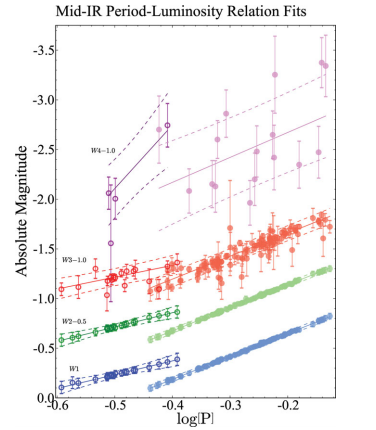
\includegraphics[width=3in]{figures/PL_relation}}
\caption{\it \small{Period-Luminosity relationship of RR Lyrae variable stars. \label{fig:plrelationrrlyrae}}}
  \end{center}
\end{figure}


\subsubsection{Cepheid}

Other variable stars that will be identified are Cepheid Type 1 and Cepheid Type 2.  A typical pulsation period of Cepheid star is $1 - 50$ days Ryden et al. (2010).  These sugergiants span the F, G, and K spectral classes, with average absolute magnitudes between $M=-0.5$ and $M=-6$ Ryden et al. (2010).  The PL relation of Cepheid Type 1 and Cepheid Type 2 is shown in Figure~\ref{fig:cephPL}. From the PL relation we can extract distances Ngeow et al. (2013). Using $m=16$, 20 s exposures will allow for photometric accuracy of $10\%$.  A Hertzsprung-Russell diagram of pulsating variable stars is shown by Figure~\ref{fig:var-star-hr} Turner et al. (2012). (\textit{Relatively young, star formation epoch?}). Cepheid variables are relatively young, a few million years, which indicates star formation regions.




\subsubsection{Spatial Distribution of Variable Stars}

Since Cepheid variables are young, it stays near star formation regions, while RR Lyrae stars are old and may move away from star formation regions. The spatial deviations of RR Lyrae stars from star formation regions indicate the structure history and dynamics of spiral arms.

%\begin{itemize}
%	\item{} Typical pulsation periods of 1-50 days - need CITATION
	%\item{} F, G, K
	%\item{} Supergiant
	%\item{} Average absolute magnitude -0.5 - -6
	%\item{} All above from B. Ryden and B. Peterson, Foundations of Astrophysics, Pearson, 2010.
	%\item{} Period to Luminosity relations in Ngeow et al. 
	%\item{} From the period to luminosity relations, distance range with $m=15$
%	\item{} Relatively young, star formation epoch?
%\end{itemize}





% side by side figures

\begin{figure}[H]
\centering
\begin{subfigure}{.5\textwidth}
  \centering
  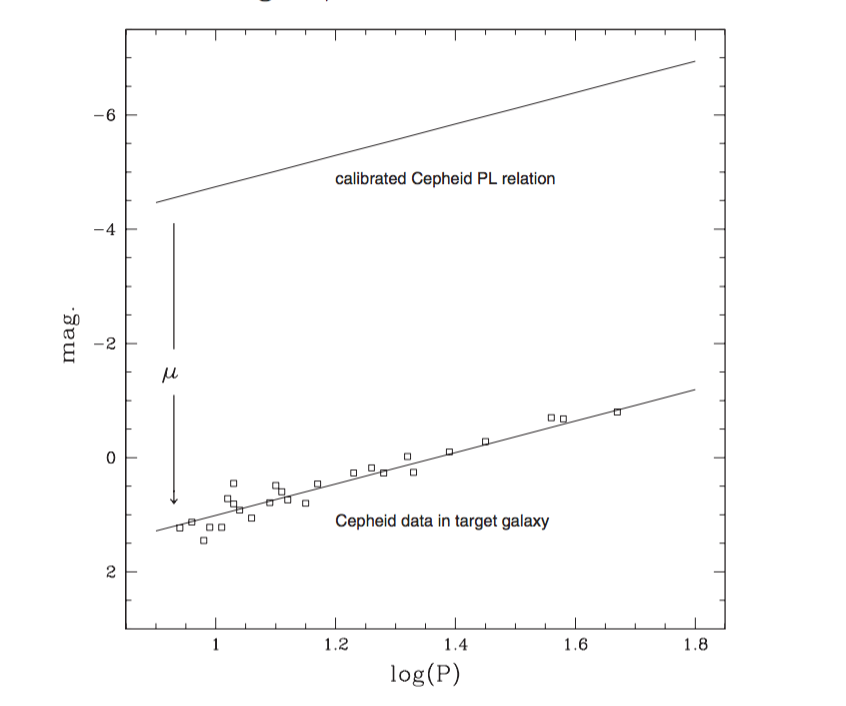
\includegraphics[width=.9\linewidth]{figures/Ngeow1_fig}
  \caption{Period-Luminosity relationship.}
  \label{fig:cephPL}
\end{subfigure}%
\begin{subfigure}{.5\textwidth}
  \centering
  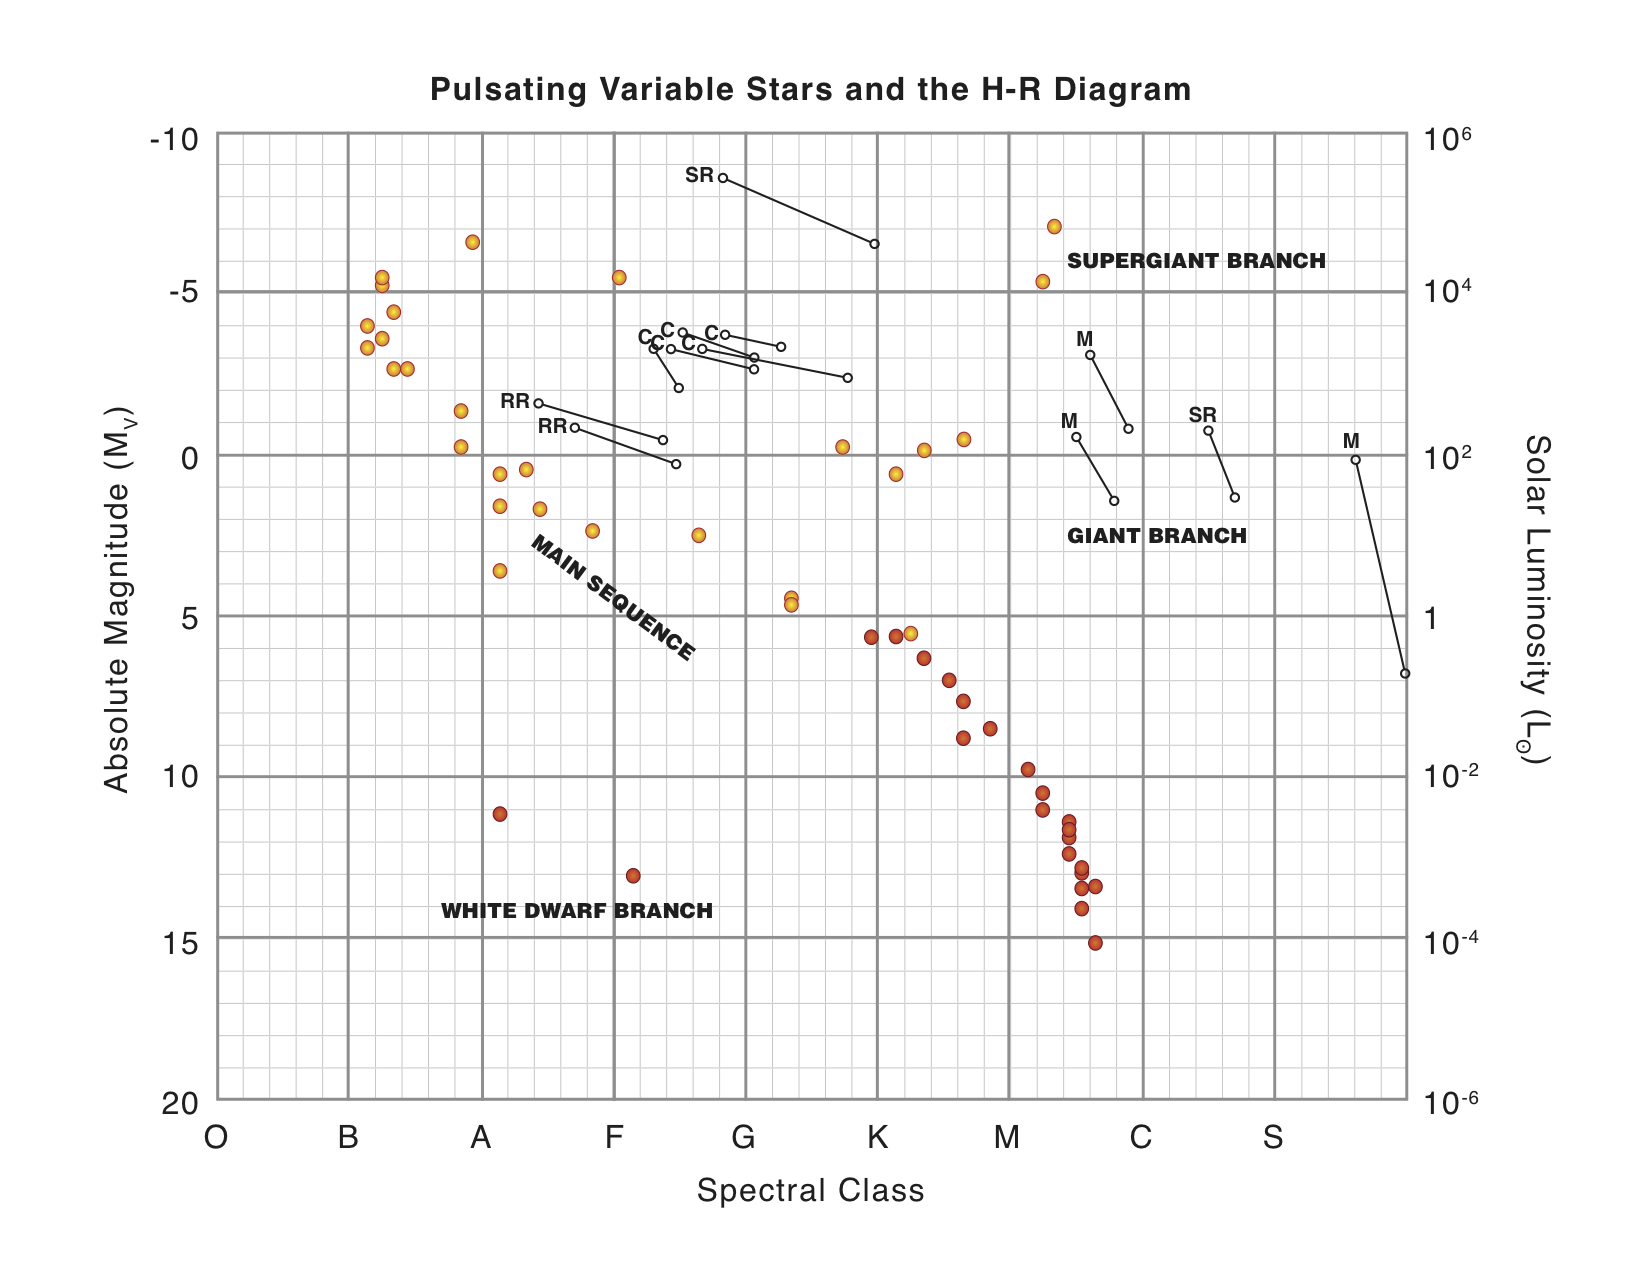
\includegraphics[width=.9\linewidth]{figures/var_star_HR.png}
  \caption{HR-Diagram of pulsating variable stars.}
  \label{fig:var-star-hr}
\end{subfigure}
\caption{Cepheid Type 1 and Cepheid Type 2 stars.}
\label{fig:test}
\end{figure}

\iffalse
\begin{figure}[H]%[htb!]
  \begin{center}
\centerline{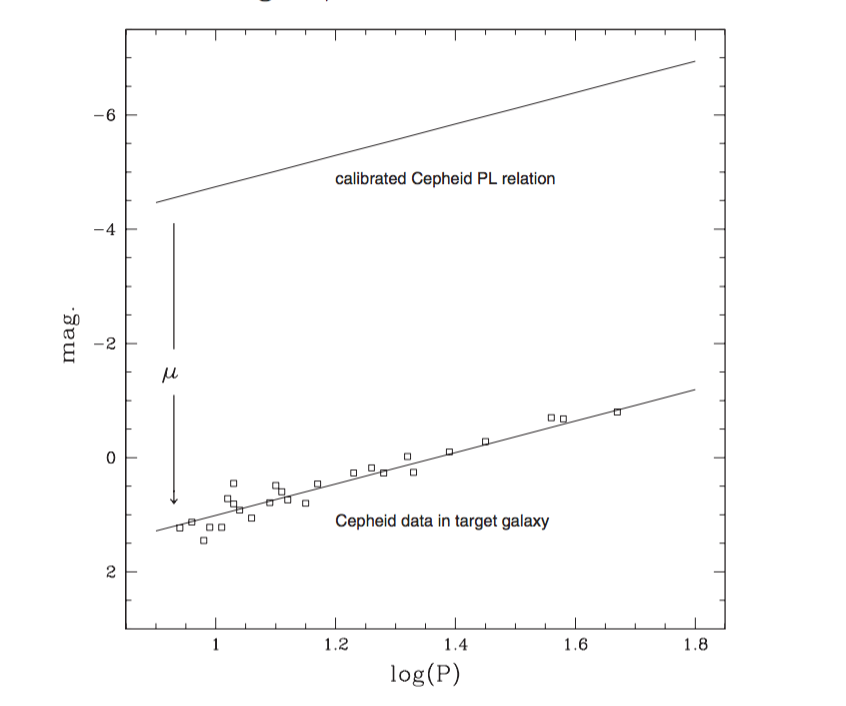
\includegraphics[width=3in]{figures/Ngeow1_fig}}
\caption{\it \small{Period to Luminosity relations of Cepheid stars. \label{fig:cephPL}}}
  \end{center}
\end{figure}

\end{figure}
\begin{figure}[H]%[htb!]
  \begin{center}
\centerline{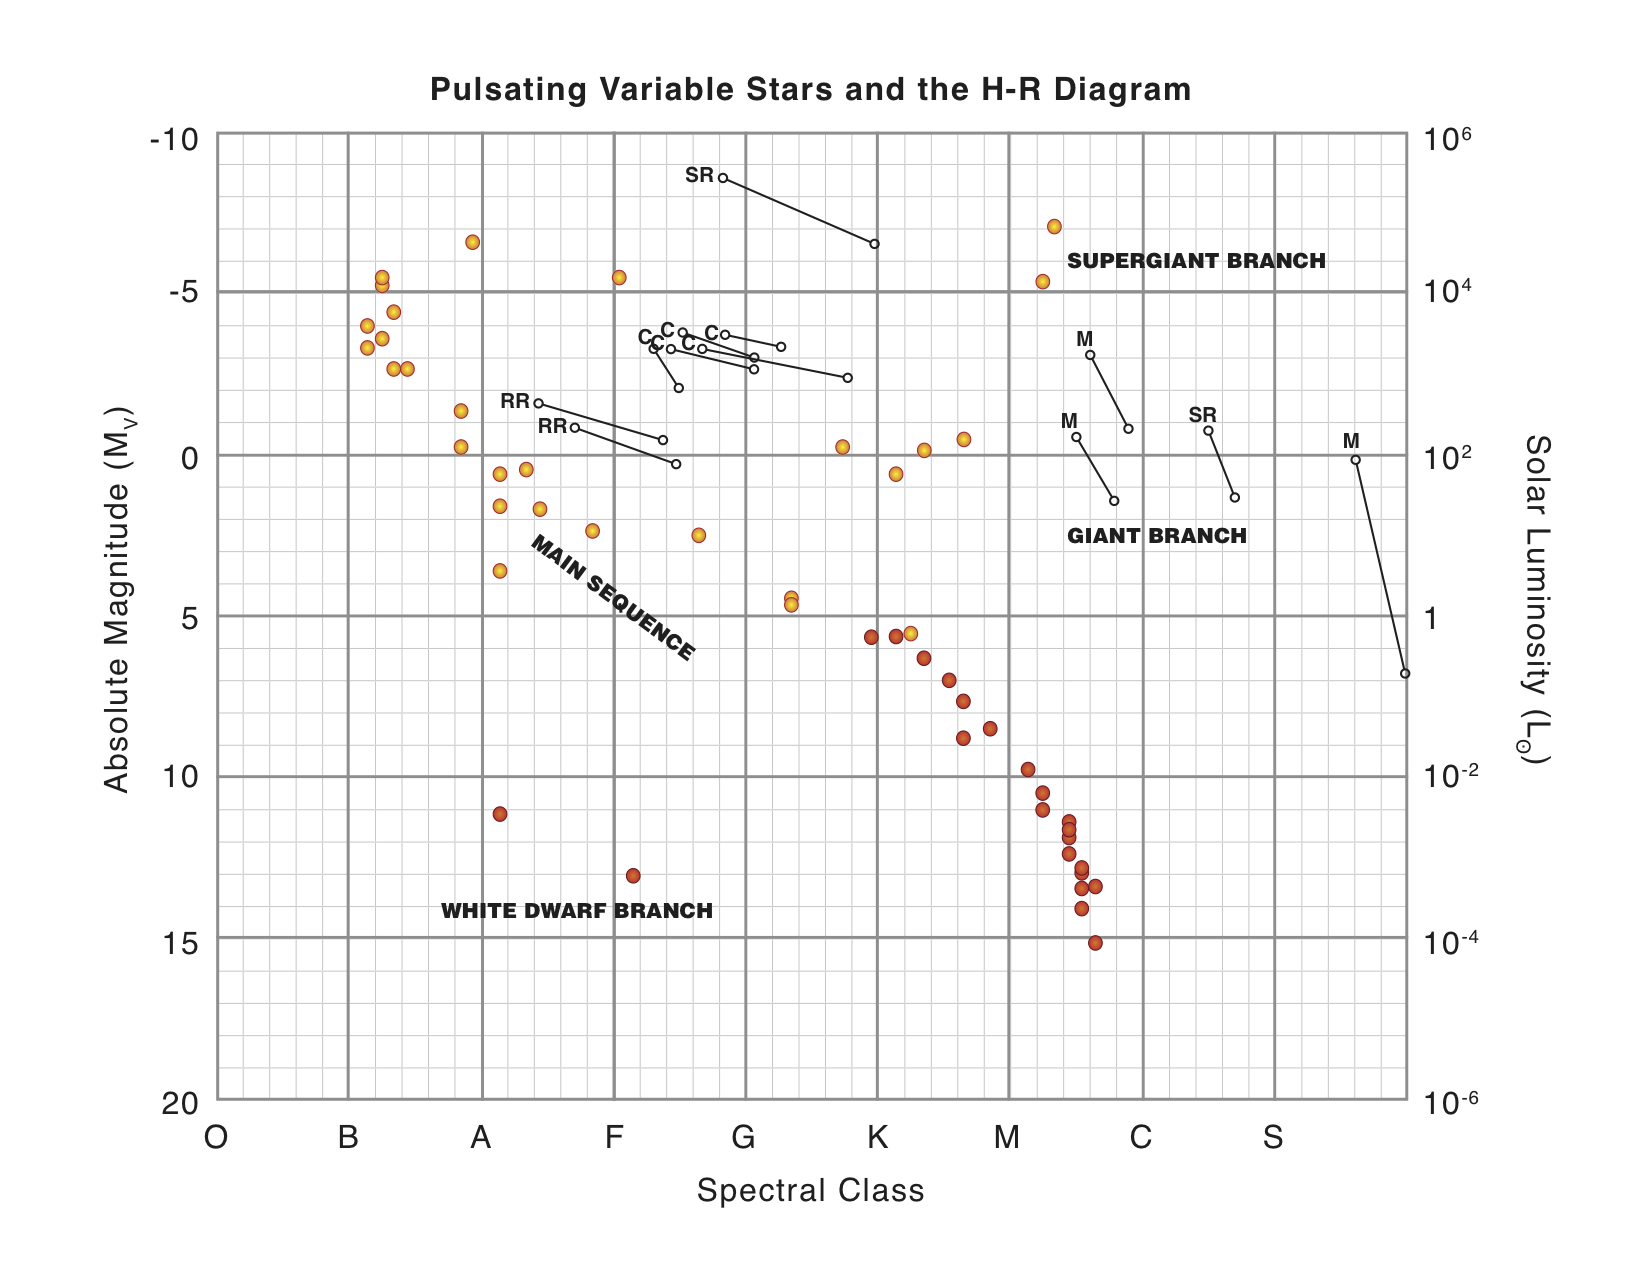
\includegraphics[width=3in]{figures/var_star_HR.png}}
\caption{\it \small{HR-Diagram: Pulsating Variable Stars. \label{fig:var-star-hr}}}
  \end{center}
\end{figure}
\fi



\subsubsection{ISM}

Near the galactic center, ISM is dense, and the number density of stars is high, which makes optical investigations quite difficult. Figure~\ref{fig:gas} shows the distribution of gasses in the Milky Way (Nakanishi and Sofue 2015). In order to determine the spiral arm structure of the Milky Way galaxy, we will avoid the galactic center. To take into account for the ISM extinction, we will use the ratio of total to selective extinction $R = \frac{1}{(\tau_{1} / \tau_{2}) -1} = \frac{1}{(\lambda_{eff,2} / \lambda_{eff,1}) \, -1}$ assuming the optical depth $\tau \propto \lambda^{-1}$ according to the Mie scattering for $\lambda < D$ where the $D$ is the dimension of a dust grain (Ryden et al. 2010 $\&$ Carroll et al. 2007). 

\begin{figure}[H]
  \begin{center}
\centerline{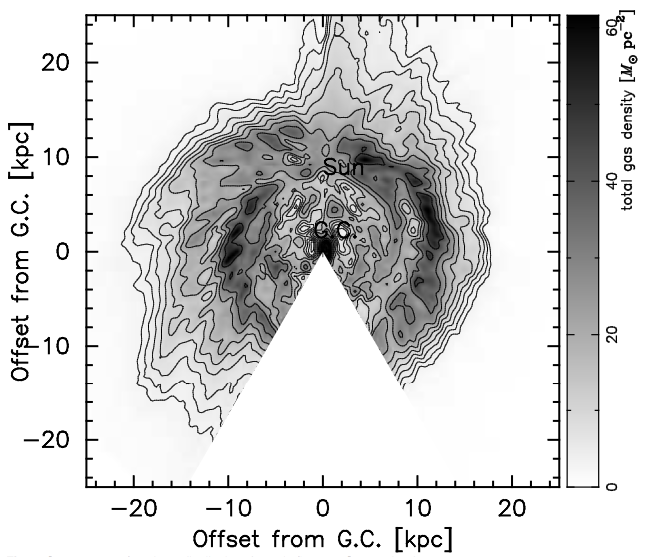
\includegraphics[width=3in]{figures/Gas.png}}
\caption{\it \small{Column density distribution of the sum of HI and H$_2$ gases. \label{fig:gas}}}
  \end{center}
\end{figure}

\noindent To test a distance measuring method using ISM, we will use observed raw data without using the ratio of total to selective extinction. From observed periods of variable stars, the absolute magnitudes can be calculated. From the calculated absolute magnitude and catalog distances, obtained by parallax, the absolute magnitudes at g,r, and i can be estimated. By comparing the estimated absolute magnitudes and calculated absolute magnitudes from the raw data, we can estimate the amount of ISM. Assuming the amount of ISM near the variable stars are similar, the distances to star near variable stars can be determined.


\clearpage
\section*{References}

\noindent\smallskip{\small
Abazajian, K. N., Adelman-McCarthy, J. K., Agu ̈eros, M. A.,\ et al. 2009, ApJS, 182, 543 \\}

\noindent\smallskip{\small
Allen, S.\ et al., 2016. (n.d.). The Classification of Stellar Spectra. Retrieved February 15, 2016, from \url{http://www.star.ucl.ac.uk/~pac/spectral_classification.html} \\}

\noindent\smallskip{\small
Asteroid Terrestrial-impact Last Alert System. (2010). Retrieved March 01, 2016, from \url{http://fallingstar.com/home.php} \\}

\noindent\smallskip{\small
B.\ et al., 2012. Types of Variables | AAVSO. Retrieved February 16, 2016, from \url{https://www.aavso.org/types-variables} \\}

\noindent\smallskip{\small
Nakanishi, H. and Sofue, Y., 2015. Three-Dimensional Distribution of the ISM in the Milky Way Galaxy: III. The Total Neutral Gas Disk. \textit{Publ. Astron. Soc. Japan (2014) 00(0), 1–14}. Retrieved February 15, 2016. \\}

\noindent\smallskip{\small
Ngeow, C.\ et al., 2013. "Distance Determination From The Cepheid And RR Lyrae Period-Luminosity Relations". \textit{Proc. IAU} 9.S301: 123-128. Web. 18 Feb. 2016. \\}

%\noindent\smallskip{\small
%Ochsenbein F., Bauer P., Marcout J., et al. 2000, A&AS 143, 221 \\}
\noindent\smallskip{\small
Ochsenbein, F., Bauer, P., Marcout, J.,\ et al. 2000, A\&AS 143, 221 \\}

\noindent\smallskip{\small
Ryden, B.\  et al., 2010. Foundations of astrophysics. San Francisco: Addison-Wesley. \\}

\noindent\smallskip{\small
Tsujimoto\ et al., 1998. The Absolute Magnitude of RR Lyrae Stars Derived from the [ITAL]Hipparcos[/ITAL] Catalogue. \textit{The Astrophysical Journal, 492}(1). Retrieved February 15, 2016. \\}

\noindent\smallskip{\small
Turner, R.\ et al., 2012. H-R Diagram Education Materials | AAVSO. Retrieved February 14, 2016, from \url{https://www.aavso.org/hr-diagram-education-materials} \\}

\noindent\smallskip{\small
Carroll, B.\  et al., 2007. An Introduction to Modern Astrophysics. San Francisco: Pearson Addison-Wesley. \\}

\noindent\smallskip{\small
Molnár, L.\  et al., 2015. Pushing the limits, episode 2: K2 observations of extragalactic RR Lyrae stars in the dwarf galaxy Leo IV 
ApJ, 812, 2, 2015, arXiv:1508.05587  \\}

\noindent\smallskip{\small
Lomb, N.R. 1976. Least-Squares Frequency Analysis of Unequally Spaced Data, Astrophysics and Space Science, vol. 39, pp. 447–462.  \\}

\noindent\smallskip{\small
Scargle, J.D. 1982 Studies in Astronomical Time Series Analysis II. Statistical Aspects of Spectral Analysis of Unevenly Sampled Data, Astrophysical Journal, vol. 263, pp. 835–853. \\}




\clearpage
\section*{TECHNICAL JUSTIFICATION}


We request 6~hours a night for 15~nights, using Pathfinder to obtain g, r, and i imaging for variable stars in the galactic plane.

\vspace{3mm} %3mm vertical space

\noindent To calculate an appropriate sampling frequency, a typical RR Lyrae star, EPIC ID 210282474, was used (Molnár et al. 2015) with artificially introduced gaps following the Gaussian distribution. Since sampling in astronomy is always uneven, we used the Lomb-Scargle analysis (Lomb 1976~$\&$~Scargle~1982). The light curve of 210282474 is shown in Figure~\ref{fig:Lcurve}, and Lomb-Scargle power plots with various sampling conditions are shown in Figures~\ref{fig:1510},~\ref{fig:1010}, and~\ref{fig:1505}. We want a distinguishable and narrow peak in power plots. To determine distances from the PL relations with $\simeq5\%$ accuracy, we need peaks with FWHM~$ \simeq 0.02$ days. From this condition, it looks like 15 nights with 10 observations/night is the lower limit sampling rate. The uncertainty in magnitude was taken to be $10\%$, and the changes, $1\% - 10\%$, in the uncertainty did not affect the period determinations significantly; we only need $10\%$ photometry.

\begin{figure}[H]
\centering
\begin{subfigure}{.5\textwidth}
  \centering
  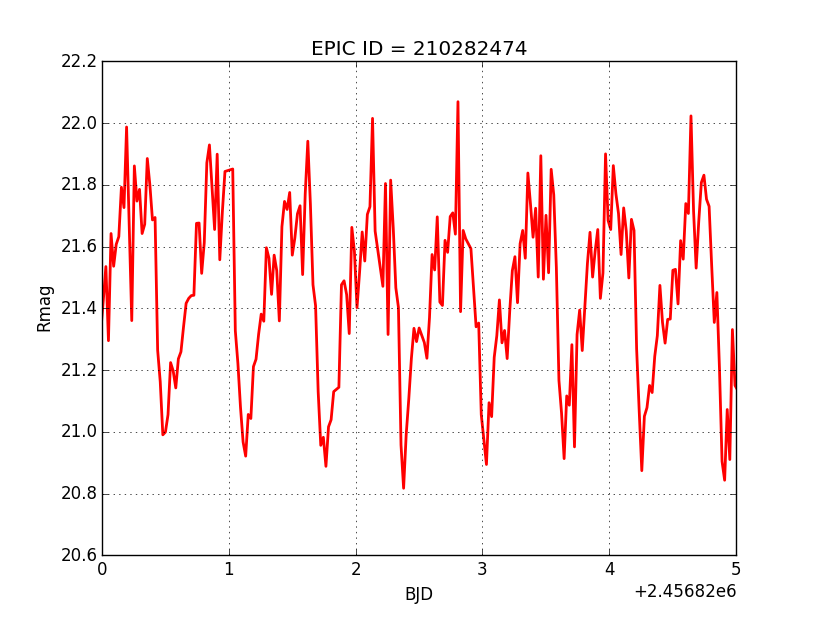
\includegraphics[width=.9\linewidth]{figures/EPICID.png}
  \caption{Light curve of 210282474.}
  \label{fig:Lcurve}
\end{subfigure}%
\begin{subfigure}{.5\textwidth}
  \centering
  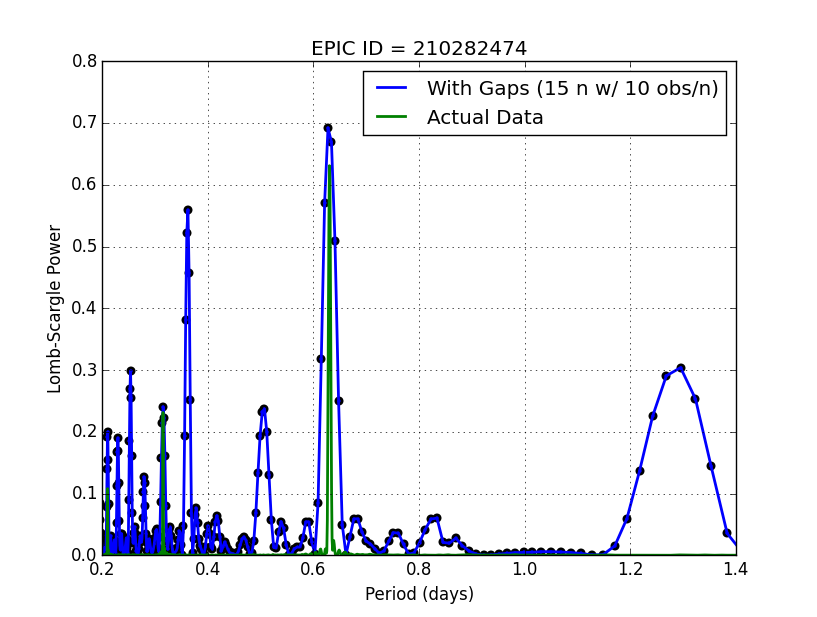
\includegraphics[width=.9\linewidth]{figures/1510Actual.png}
  \caption{Power plot with 15 nights with 10 observations/night.}
  \label{fig:1510}
\end{subfigure}
\begin{subfigure}{.5\textwidth}
  \centering
  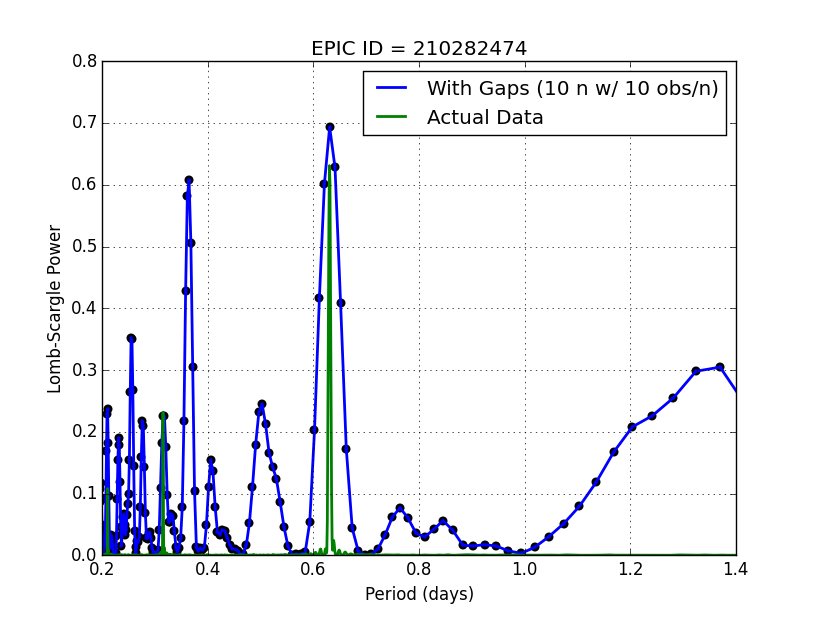
\includegraphics[width=.9\linewidth]{figures/1010Actual.png}
  \caption{Power plot with 10 nights with 10 observations/night.}
  \label{fig:1010}
  \end{subfigure}%
  \begin{subfigure}{.5\textwidth}
  \centering
  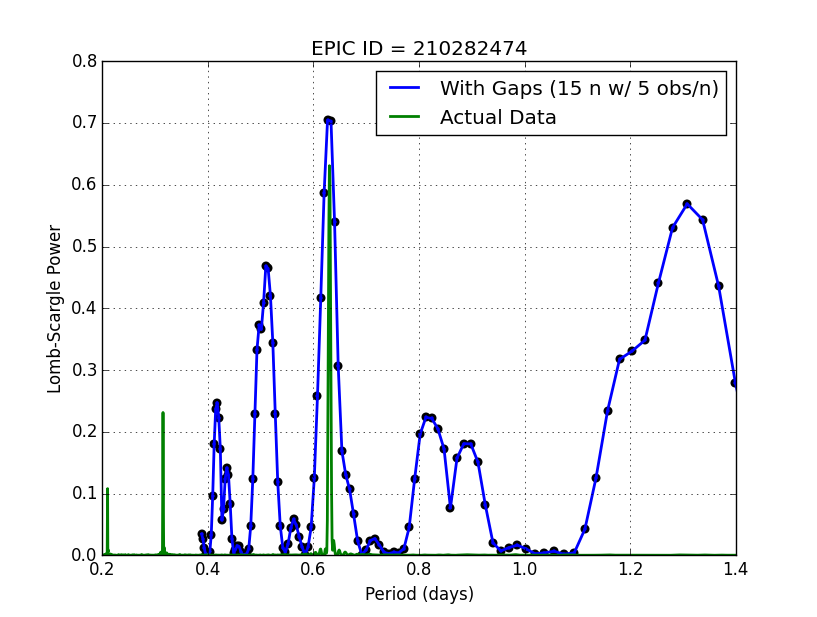
\includegraphics[width=.9\linewidth]{figures/1505Actual.png}
  \caption{Power plot with 15 nights with 5 observations/night.}
  \label{fig:1505}
\end{subfigure}
\caption{EPIC ID 210282474.}
\label{fig:EPIC}
\end{figure}


\noindent For $m_g = m_r = 16$ and $m_i = 15.7$, an exposure time of $20$~sec yields $10\%$ photometry. We want to cover the galactic plane, $165^{\circ}~<~l~<~195^{\circ}$ and $b=\pm10^{\circ}$ avoiding the galactic center and the sun. With the magnitudes, exposure time, and size of the field, we request $6$ hr/night for $15$ nights, resulting the total observational time of $90$~hr.  

%$90\deg < l <330\deg$ and $-2 \deg < b < 2 \deg$ avoiding the galactic center and the sun. With the magnitudes, exposure time, and size of the field, we request $1.5$ hr/night for $15$ nights, resulting the total observational time of $22.5$~hr.  


\vspace{3mm} %3mm vertical space


\noindent Since typical pulsation periods of Cepheid variables are longer than that of RR Lyrae stars, we would be able to sample Cepheid light curves as well by using the sampling rate discussed above. 



\section{Observation Specifics}
In order to achieve photometric accuracy of $10\%$ and $SNR~=~10$, seeing conditons must not exceed 1.5~$arcsec$ during the collection of each 20~$s$ exposure.  Pathfinder residing on Mauna Loa minimizes chances of poor seeing conditions.  The sky transparency for each filter are $\mu^{sky}_{g}~=~21.9$, $\mu^{sky}_{r}~=~21.0$, $\mu^{sky}_{i}~=~20.1$ Asteroid et al. (2010).  Better observing conditions occur as light from the Moon is minimized, making nights containing the New Moon ideal.  A New Moon will occur on March 9$^{th}$ and April 7$^{th}$.  Due to upcoming dedlines, it is requested that observations occur in the nights surrounding the March 9$^{th}$  New Moon.  The minimum requirement is to avoid a Full Moon, which will occur on March 23$^{rd}$ or April 22$^{nd}$.\\

%$b=\pm10^{\circ}$ gives better spatial resolution but less stars

\noindent To properly measure the Milky Way only a portion of the galactic plane needs to be observed, bound by $165^{\circ}~<~l~<~195^{\circ}$ at $b=\pm 5^{\circ}$.  Starting with $l~=~165^{\circ}$ centered at $b=5^{\circ}$, data will be gathered using g, then r, then i filters.  Once data from each filter is recorded, the FOV will be shifted by 3~$^{\circ}$.  Observations in each of the three filters will be recorded, then the FOV shifted by another 3~$^{\circ}$.  Once $l~=~195$ is reached, the FOV will move to center around $b=-5^{\circ}$.  Data collected by changing filters before moving the FOV will reduce potential aliasing.  To collect the necessary data, we will need 6~hours a night for 15~nights.  During each 6~hour time slot, 10 observations will be made.  With the addition of overhead time, a total of 22 exposures will be recorded each night.

\section*{LIST OF PRINCIPAL OBJECTS \emph{(to be studied in run justified above)}}
\begin{table}[H]\label{tab:collabs}
	\begin{center}
		%\caption{\it \small{[title]}}
		\resizebox{\columnwidth}{!}{%
	\begin{tabular}{ | c | c | c | c | c | c | } \hline
		Program & Object & RA~(deg) & Dec~(deg) & Mag~(specify band) & Exposure Time~(s) \\ \hline
	    A & Galactic Plane & 81.60342023 &  44.25952438 & $m_{g}=16$ & 20 \\ \hline
	    A & Galactic Plane & 81.60342023 &  44.25952438 & $m_{r}=16$ & 20 \\ \hline
	    A & Galactic Plane & 81.60342023 &  44.25952438 & $m_{i}=15.7$ & 20 \\ \hline
	    A & Galactic Plane & 83.82934318 & 41.75280277 & $m_{g}=16$ & 20 \\ \hline
	    A & Galactic Plane & 83.82934318 & 41.75280277 & $m_{r}=16$ & 20 \\ \hline
	    A & Galactic Plane & 83.82934318 & 41.75280277 & $m_{g}=15.7$ & 20 \\ \hline
	    %A & Galactic Plane & 85.90167981 &  39.2133976 & m \\ \hline
	    %A & Galactic Plane & 87.84305649 & 36.64669143 & m \\ \hline
	    %A & Galactic Plane & 89.6728044 & 34.05719814 & m \\ \hline
	    %A & Galactic Plane & 91.40752288 &  31.44874046 & m \\ \hline
	    %A & Galactic Plane & 93.06155626 &  28.82459032 & m \\ \hline
	    %A & Galactic Plane & 94.64739347 &  26.18758049 & m \\ \hline
	    %A & Galactic Plane & 96.17600119 &  23.54019392 & m \\ \hline
	    %A & Galactic Plane & 97.6571018 & 20.88463602 & m \\ \hline
	    %A & Galactic Plane & 99.09940579 &  18.22289366 & m \\ \hline
	\end{tabular}
	}
	\end{center}
\end{table}

\iffalse
\section*{Things to Discuss Further}

\begin{itemize}
	%\item{} Use gri data to identify variable Stars 		
	%\item{} Use Period-Luminosity relationship to get distance 
	%\item{} Map 3D spatial distribution
	%\item{} Distance Equation
	\item{} Determine deviation of variable stars from model
	\item{} Variations arise from gravitational effects from unknown sources
	\item{} Figure out dark matter distribution
	\item{} include - Plot of known var star distributions in spiral arms
	\item{} comment on knowing m from tying into pan-starrs
	\item{} difference in 3 variable stars light curves - show examples
\end{itemize}

\begin{itemize}
	\item{} Use catalogs to map known variable star locations
	\item{} Cepheid or RR Lyrae? - Focus on RR Lyrae
	\item{} gri data will be supplemental - identifying previously unknown variable stars
	\item{} More specificity
	\item{} Refine overall question
	%\item{} clarify big picture Q
	\item{} What are Apparent and Absolute magnitudes
	\item{} Sampling necessary to properly describe lightcurve (how often, how long)
\end{itemize}
\fi



\end{document}